\pagestyle{circuito}
\label{circuito}

\hspace{.5cm}

\begin{center}
\hspace*{-2.5cm}\raisebox{5.5cm}{\rotatebox[origin=t]{90}{\Formular{\textbf{Lançamento}}}}
\hspace{2cm}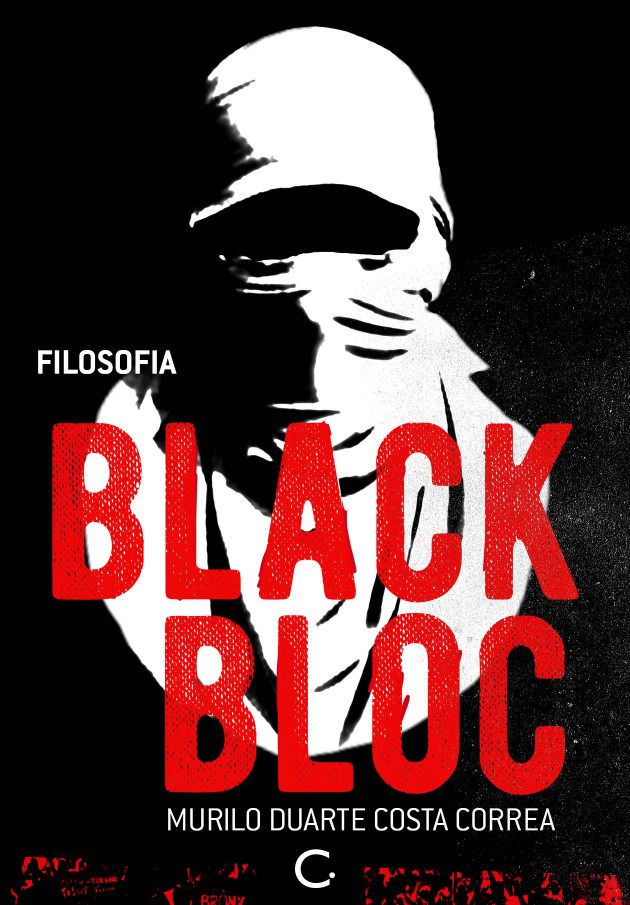
\includegraphics[width=45mm]{./imgs/blackbloc.jpg}
\end{center}

\hspace*{-2cm}\_\_\_\_\_\_\_\_\_\_\_\_\_\_\_\_\_\_\_\_\_\_\_\_\_\_\_\_\_\_\_\_\_\_\_\_\_\_\_\_\_\_\_\_\_\_\_\_\_\_\_\_\_\_\_\_\_\_\_\_\_\_\_\_\_\_\_\_\_\_\_\_\_\_

\medskip

\noindent{}Em junho de 2013, na maior erupção social recente, o Black bloc ganhou os holofotes como nova prática de luta. Analistas foram forçados a compreendê"-lo, normalmente municiando um repertório conceitual que não o entendia em seus próprios termos. {\slsc{Filosofia Black bloc}} procura suprir essa carência e conceber um arcabouço teórico que permita abordar o Black bloc como fenômeno. Produzir, no pensamento, uma filosofia Black bloc.

\hspace{.5cm}

\hspace*{-.4cm}\begin{minipage}[c]{0.45\linewidth}
\small{
{\Formular{\textbf{
\hspace*{-.1cm}Título: Filosofia Black bloc\\
Autor: Murilo D. C. Correa\\ 
Editora: Circuito\\
Páginas: 166\\
Formato: 12,7x19,1cm\\
Preço: R\$ 46,90\\
}}}}
\end{minipage}
\begin{minipage}[c]{0.50\linewidth}
\small{``Se quisermos levar Junho a sério, é preciso levar o black bloc a sério e produzir um modo do pensamento que corresponda ao fenômeno. Não perguntar `o que é o black bloc?', mas como o black bloc nos violenta a pensar.''} 
\end{minipage}

\pagebreak

\hspace{.5cm}

\begin{center}
\hspace*{-.5cm}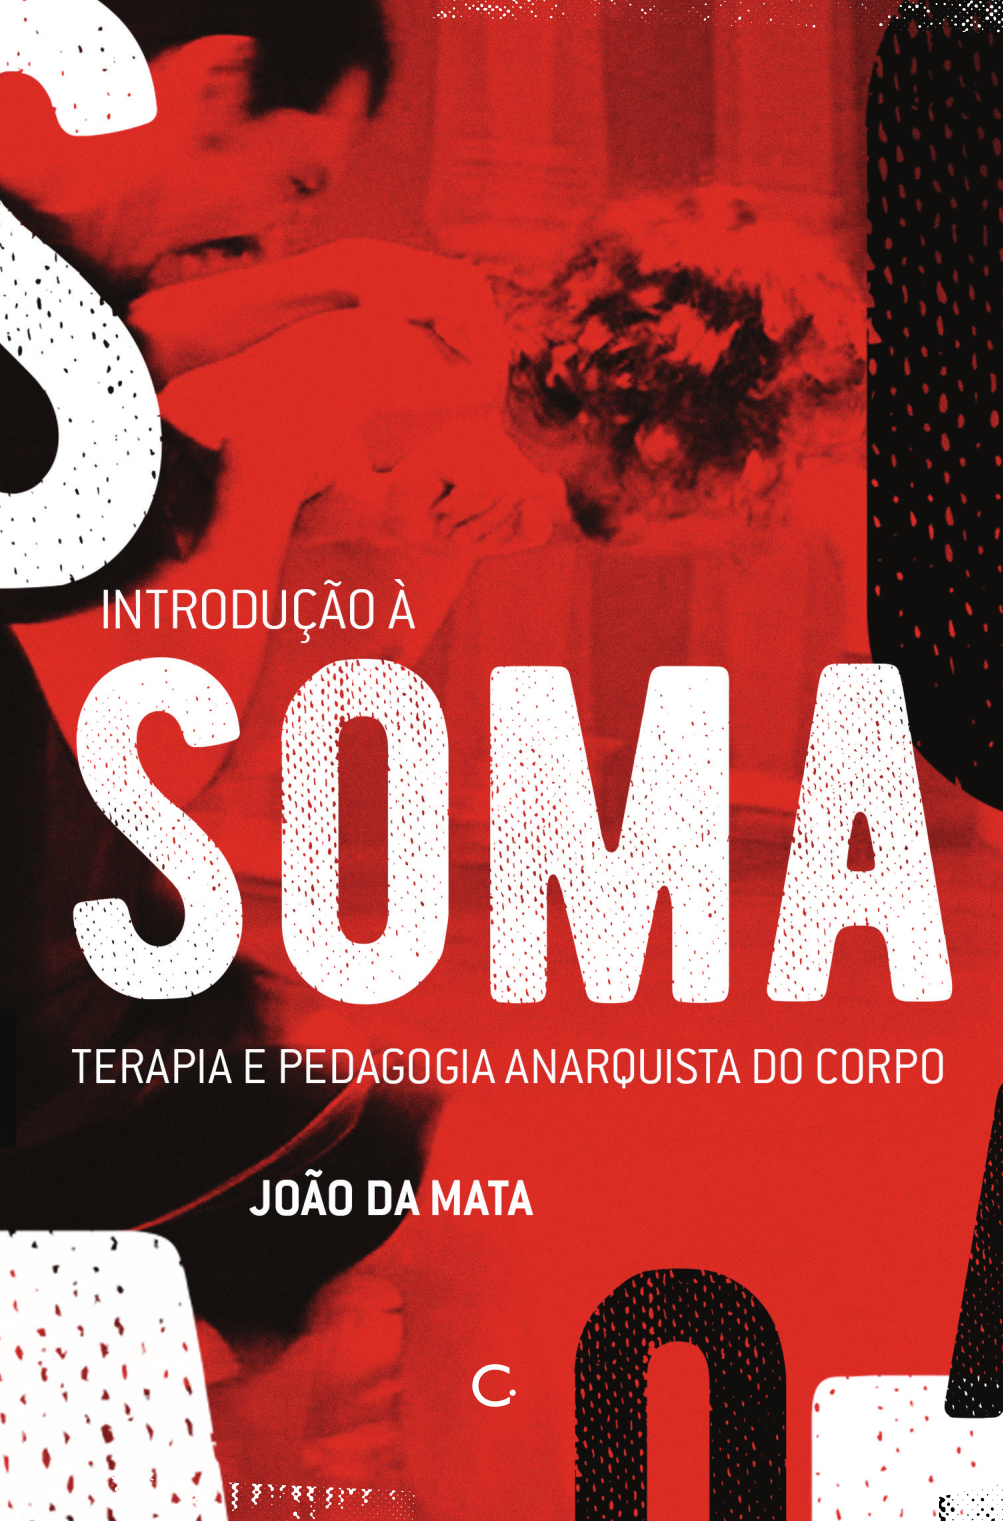
\includegraphics[width=45mm]{./imgs/soma.jpg}
%\hspace*{6cm}\raisebox{2cm}{\rotatebox[origin=t]{90}{\Formular{\textbf{Lançamento}}}}
\end{center}

\hspace*{-2cm}\_\_\_\_\_\_\_\_\_\_\_\_\_\_\_\_\_\_\_\_\_\_\_\_\_\_\_\_\_\_\_\_\_\_\_\_\_\_\_\_\_\_\_\_\_\_\_\_\_\_\_\_\_\_\_\_\_\_\_\_\_\_\_\_\_\_\_\_\_\_\_\_\_\_

\medskip

\noindent{}{\slsc{Introdução à \scalebox{.8}{SOMA}}} trata de um processo terapêutico realizado em grupo, corporal, que busca no pensamento anarquista uma crítica às formas de poder impregnadas no comportamento individual. O grupo funciona como um micro"-laboratório social, daí sua originalidade: a terapia é criação de si, em que a construção das práticas de liberdade é o antídoto para os conflitos gerados pelas hierarquias sociais.

\hspace{.5cm}

\hspace*{-.4cm}\begin{minipage}[c]{0.45\linewidth}
\small{
{\Formular{\textbf{
\hspace*{-.1cm}Título: Introdução à \scalebox{.8}{SOMA}: terapia e pedagogia anarquista do corpo\\
Autor: João da Mata\\ 
Editora: Circuito\\
Páginas: 106\\
Formato: 12,7x19,1cm\\
Preço: R\$ 42,90\\
}}}}
\end{minipage}
\begin{minipage}[c]{0.50\linewidth}
\small{Lorem ipsum dolor sit amet, consectetur adipiscing elit.
Donec sodales tortor a purus accumsan, ut ultricies. Lorem ipsum dolor sit amet, consectetur adipiscing elit. Lorem ipsum dolor sit amet. Lorem ipsum dolor sit amet.} 
\end{minipage}

\pagebreak

\hspace{.5cm}

\begin{center}
\hspace*{-1cm}\raisebox{5.5cm}{\rotatebox[origin=t]{90}{\Formular{\textbf{Lançamento}}}}
\hspace{1cm}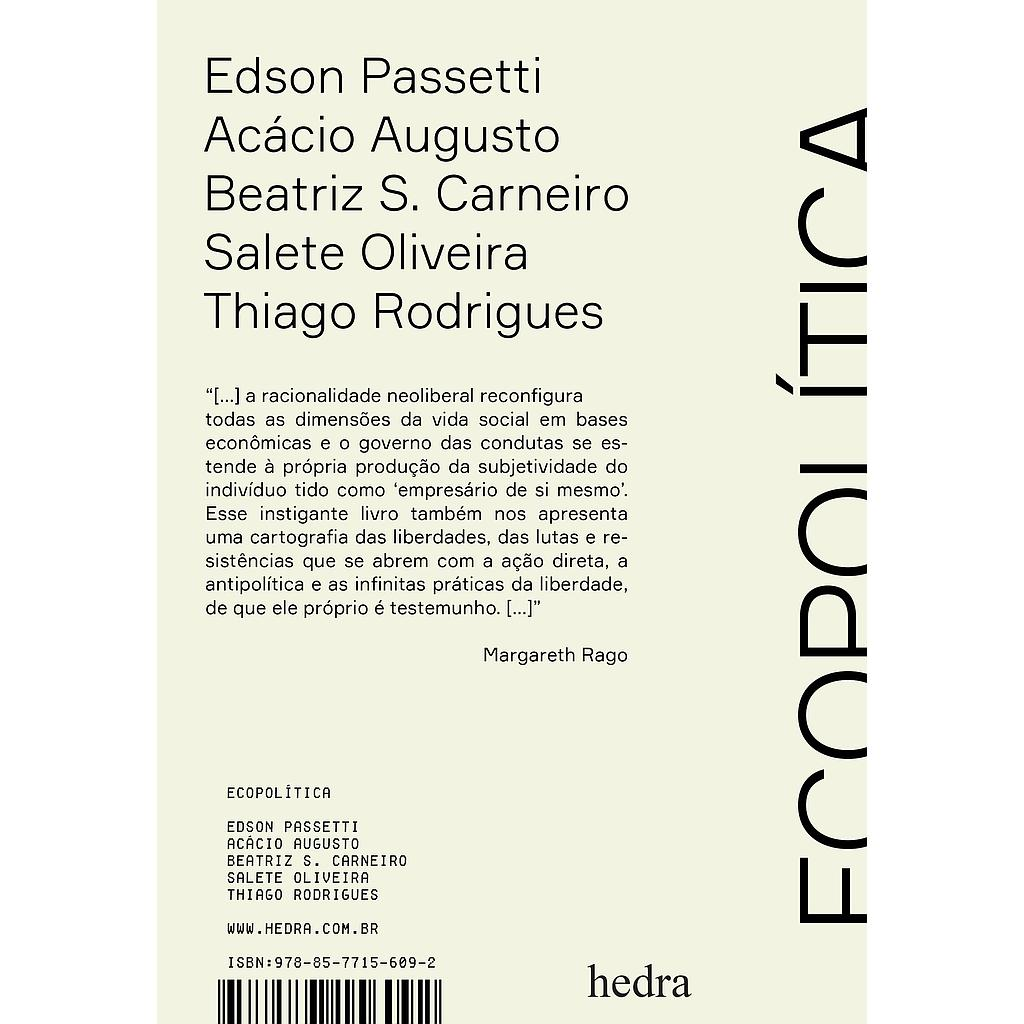
\includegraphics[width=70mm]{eco.jpeg}
\end{center}

\hspace*{-2cm}\_\_\_\_\_\_\_\_\_\_\_\_\_\_\_\_\_\_\_\_\_\_\_\_\_\_\_\_\_\_\_\_\_\_\_\_\_\_\_\_\_\_\_\_\_\_\_\_\_\_\_\_\_\_\_\_\_\_\_\_\_\_\_\_\_\_\_\_\_\_\_\_\_\_

\medskip

\noindent{}Lorem ipsum dolor sit amet, consectetur adipiscing elit.
Donec sodales tortor a purus accumsan, ut ultricies purus
maximus. Aliquam bibendum consequat mi, sed commo-
do velit pellentesque id. Vivamus ultricies ligula in semper
sagittis. Donec mollis odio in lectus tristique, sed convallis
est interdum. Cras eget sem condimentum, pretium purus
eu, auctor.

\hspace{.5cm}

\hspace*{-.4cm}\begin{minipage}[c]{0.45\linewidth}
\small{
{\Formular{\textbf{
\hspace*{-.1cm}Título: Ecopolítica\\
Autor: Edson Passetti\\ 
Editora: Hedra\\
Páginas: 476\\
Formato: 23x16cm\\
Preço: R\$ 79,90\\
}}}}
\end{minipage}
\begin{minipage}[c]{0.50\linewidth}
\small{Lorem ipsum dolor sit amet, consectetur adipiscing elit.
Donec sodales tortor a purus accumsan, ut ultricies. Lorem ipsum dolor sit amet, consectetur adipiscing elit. Lorem ipsum dolor sit amet. Lorem ipsum dolor sit amet.} 
\end{minipage}

\pagebreak

\hspace{.5cm}

\begin{center}
\hspace*{-.5cm}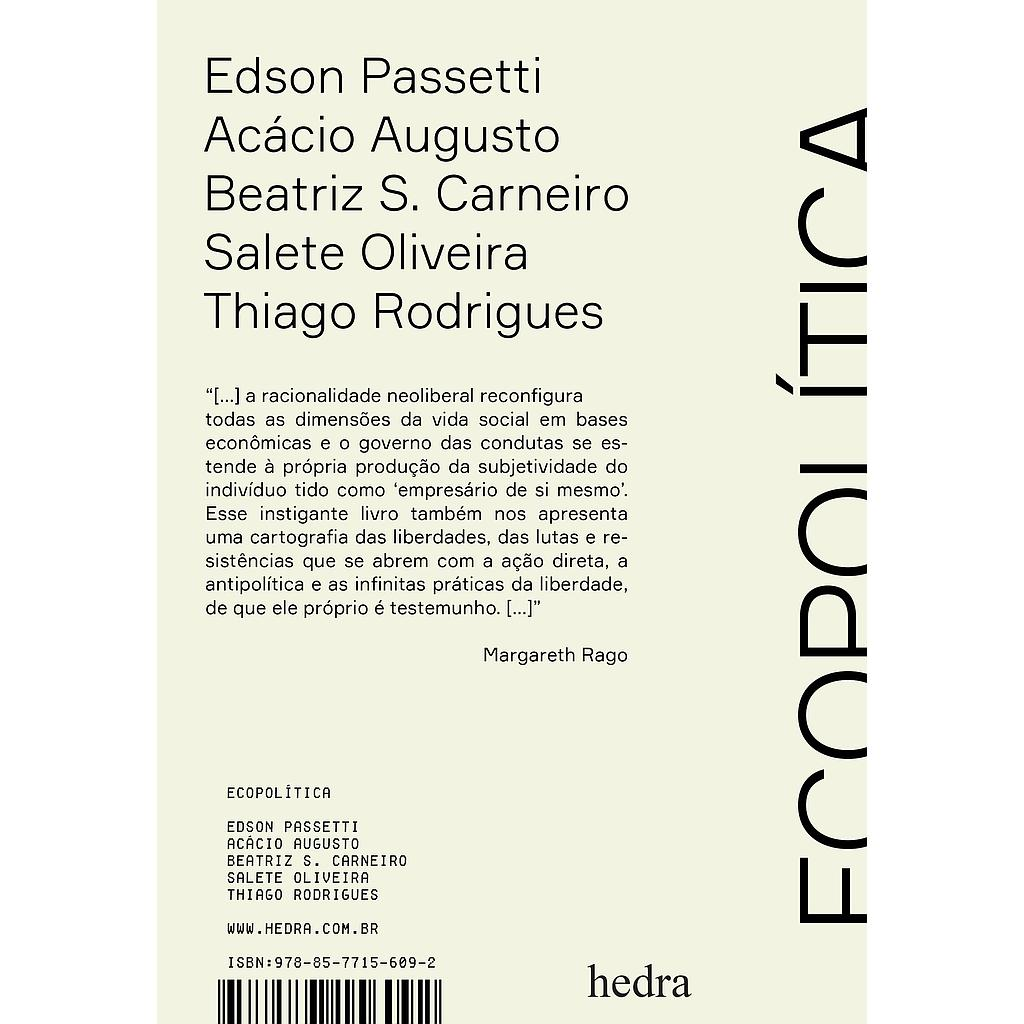
\includegraphics[width=70mm]{eco.jpeg}
%\hspace*{6cm}\raisebox{2cm}{\rotatebox[origin=t]{90}{\Formular{\textbf{Lançamento}}}}
\end{center}

\hspace*{-2cm}\_\_\_\_\_\_\_\_\_\_\_\_\_\_\_\_\_\_\_\_\_\_\_\_\_\_\_\_\_\_\_\_\_\_\_\_\_\_\_\_\_\_\_\_\_\_\_\_\_\_\_\_\_\_\_\_\_\_\_\_\_\_\_\_\_\_\_\_\_\_\_\_\_\_

\medskip

\noindent{}Lorem ipsum dolor sit amet, consectetur adipiscing elit.
Donec sodales tortor a purus accumsan, ut ultricies purus
maximus. Aliquam bibendum consequat mi, sed commo-
do velit pellentesque id. Vivamus ultricies ligula in semper
sagittis. Donec mollis odio in lectus tristique, sed convallis
est interdum. Cras eget sem condimentum, pretium purus
eu, auctor.

\hspace{.5cm}

\hspace*{-.4cm}\begin{minipage}[c]{0.45\linewidth}
\small{
{\Formular{\textbf{
\hspace*{-.1cm}Título: Ecopolítica\\
Autor: Edson Passetti\\ 
Editora: Hedra\\
Páginas: 476\\
Formato: 23x16cm\\
Preço: R\$ 79,90\\
}}}}
\end{minipage}
\begin{minipage}[c]{0.50\linewidth}
\small{Lorem ipsum dolor sit amet, consectetur adipiscing elit.
Donec sodales tortor a purus accumsan, ut ultricies. Lorem ipsum dolor sit amet, consectetur adipiscing elit. Lorem ipsum dolor sit amet. Lorem ipsum dolor sit amet.} 
\end{minipage}

\pagebreak